\documentclass[12pt]{article}
% Full article preamble (duplicated, no common file)
\usepackage{fontspec}
\usepackage[a4paper,margin=2.5cm,includefoot]{geometry}
\usepackage{polyglossia}
\usepackage{amsmath}
\usepackage{amssymb}
\usepackage{xcolor}
\usepackage{fancyhdr}
\usepackage{graphicx}
\usepackage{listings}
\usepackage[most]{tcolorbox}
\usepackage{pifont}
\usepackage{enumitem}
\usepackage{titlesec}
\usepackage[bottom]{footmisc}
\usepackage{titling}
\usepackage{minted}
\usepackage{etoolbox}
\usepackage{array}
\usepackage{extsizes}

\newfontfamily\emoji{Segoe UI Emoji}

\pagestyle{fancy}

\setmainlanguage[numerals=western]{arabic}
\setotherlanguage{english}
\newfontfamily\arabicfont[Script=Arabic]{Amiri}
\newfontfamily\arabicfonttt[Script=Arabic]{Courier New}

\lstset{
  language=[Sharp]C,
  numbers=left,
  stepnumber=1,
  numbersep=8pt,
  frame=single,
  basicstyle=\ttfamily\small,
  keywordstyle=\color{blue},
  stringstyle=\color{red},
  commentstyle=\color{green!50!black}
}

\newif\ifdetailed
\ifdefined\setdetailed
  \setdetailed
\fi

\newif\ifwithsols
\ifdefined\setwithsols
  \setwithsols
\fi

% unified tcolorboxes for articles
\tcbset{colback=white, colframe=black, fonttitle=\bfseries, boxrule=0.8pt}
\newtcolorbox{boxDef}[1][]{colback=blue!5!white,colframe=blue!75!black,
  title={{\emoji📘} تعريف\ifx\\#1\\\else ~#1\fi :}}
\newtcolorbox{boxExercise}[1][]{colback=cyan!5!white,colframe=cyan!70!black,
  title={{\emoji🧩} تمرين\ifx\\#1\\\else ~#1\fi :}}
\newtcolorbox{boxExample}[1][]{colback=yellow!5!white,colframe=orange!90!black,
  title={{\emoji📝} مثال\ifx\\#1\\\else ~#1\fi :}}
\newtcolorbox{boxNote}[1][]{colback=gray!10!white,colframe=black,
  title={{\emoji✨} ملاحظة\ifx\\#1\\\else ~#1\fi :}}
\newtcolorbox{boxAttention}[1][]{colback=magenta!10!white,colframe=magenta!80!black,
  title={{\emoji🔔} تنبيه\ifx\\#1\\\else ~#1\fi :}}
\newtcolorbox{boxWarning}[1][]{colback=red!5!white,colframe=red!75!black,
  title={{\emoji⚡} ملاحظة هامة\ifx\\#1\\\else ~#1\fi :}}
\newtcolorbox{boxSolution}[1][]{colback=green!5!white,colframe=green!60!black,
  title={{\emoji✅} حل\ifx\\#1\\\else ~#1\fi :}}
\newtcolorbox{boxSymbol}[1][]{colback=purple!5!white,colframe=purple!70!black,
  title={{\emoji🔣} رمز\ifx\\#1\\\else ~#1\fi :}}

\tcbset{simplecode/.style={ colback=gray!5, colframe=black!50, boxrule=0.4pt, arc=2pt, left=4pt,right=4pt,top=4pt,bottom=4pt}}
\newenvironment{boxCode}{\begin{tcolorbox}[simplecode]}{\end{tcolorbox}}

\newcolumntype{C}[1]{>{\centering\arraybackslash}p{#1}}

% redefine spaces after titles
\makeatletter
\renewcommand{\@maketitle}{%
  \begin{center}
    {\huge \bfseries \@title \par}%
    \vskip 0.2em % space between title and author
    {\large \@author \par}%
    % \vskip 0.2em % space between author and date
    % {\normalsize \@date \par}%
  \end{center}
}
\makeatother

\fancyhf{} % clear default
\fancypagestyle{plain}{
  \fancyhf{}
  \fancyhead[L]{مدرسة التسامح الشاملة}
  % \fancyhead[L]{
\includegraphics[height=1cm]{../../../images/logoTasamoh.png}}
  \fancyhead[R]{الأستاذ محمود اغبارية}
  \fancyfoot[C]{\thepage}
}

\fancyhead[L]{مدرسة التسامح الشاملة}
\fancyhead[R]{الأستاذ محمود اغبارية}
\fancyfoot[C]{\thepage}
% \date{\today}

\setcounter{tocdepth}{3} % only section subsection and subsubsection in TOC


% ----------------------


% \begin{document}

% \maketitle

% % \clearpage  % start TOC on a new page
% % \renewcommand{\contentsname}{جدول المحتويات}
% % \tableofcontents
% % \clearpage

% \part*{part 1} % the * prevents numbering
% \section*{مقدمة}
% \subsection*{مثال رياضي}
% \subsubsection*{مثال فرعي}
% \paragraph*{ paragraph 1}
% \subparagraph*{sub paragraph 1}

% \ifdetailed
% \begin{english}
% \begin{minted}{csharp}
% // C# Example
% \end{minted}
% \end{english}
% \fi

% OLD WAY
% \ifdetailed
% \begin{english}
% \begin{lstlisting}
% // C# Example
% \end{lstlisting}
% \end{english}
% \fi

% % 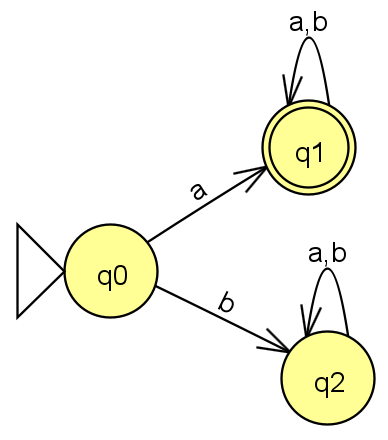
\includegraphics[width=0.2\textwidth]{../../../images/DFAs/ex1_q1.png}



% \vspace{3cm}
% \begin{flushleft}
% أرجو لكم وقتًا ممتعًا.

% الأستاذ محمود اغبارية.
% \end{flushleft}


% \end{document}


\title{وظيفة بيتية 1 للصف العاشر 10}

\begin{document}

\maketitle
\thispagestyle{fancy}

\begin{warning}
تأكد أن الكود الذي تسلمه يعمل - شغّله وافحصه قبل التسليم.
\end{warning}

\begin{note}
    تأكد من استخدام نوع المتغير الصحيح، $\mathtt{int}$ للمتغيرات التي لا تكون إلا عددًا صحيحًا، و $\mathtt{double}$ للمتغيرات التي قد تكون أعدادًا عشرية.
\end{note}

\begin{enumerate}

\vspace{1cm}
\item
اكتب برنامجًا يستقبل من المستخدم سنة ميلاده، ويطبع له كم سيكون عمره في عام 2030.
\begin{example}
\begin{english}
\begin{lstlisting}
What is your birth year?
2005
In 2030, you will be 25 years old.
\end{lstlisting}
\end{english}
\end{example}

\ifwithsols
\begin{solution}
\begin{english}
\begin{lstlisting}
private static void Main(string[] args)
{
    Console.WriteLine("What is your birth year?");
    int birthYear = int.Parse(Console.ReadLine());
    Console.WriteLine($"In 2030, you will be {2030 - birthYear} years old.");
}
\end{lstlisting}
\end{english}
\end{solution}

\clearpage

\else
\vspace{1cm}
\fi

\item
اكتب برنامجًا يستقبل من المستخدم سعر سلعة معيّنة، ثم يضيف لها الضريبة المضافة، بقدر $18\%$. \\
في النهاية اطبع للمستخدم السعر النهائي للسلعة مع الضريبة.

\begin{example}
\begin{english}
\begin{lstlisting}
Enter the price:
30
Price after adding tax is: 35.4
\end{lstlisting}
\end{english}
لأنّ $30 + 0.18 \cdot 30 = 35.4$
\end{example}

\ifwithsols
\begin{solution}
\begin{english}
\begin{lstlisting}
private static void Main(string[] args)
{
    Console.WriteLine("Enter the price:");
    double price = double.Parse(Console.ReadLine());
    Console.WriteLine($"Price after adding tax is: {price + price * 0.18}");
}
\end{lstlisting}
\end{english}
\end{solution}

\fi

\clearpage

\item
اكتب برنامجًا يستقبل من المستخدم الراتب \textbf{الشهري} لعامل ما. \\
ثم يستقبل منه قيمة الضريبة \textbf{السنوية} التي يجب دفعها. \\
ثم يستقبل من المستخدم \textbf{النسبة المئوية} للعلاوة السنوية التي حصل عليها العامل. \\
في النهاية اطبع له الراتب السنوي بعد خصم الضريبة وإضافة العلاوة
\begin{example}
\begin{english}
\begin{lstlisting}
Enter your monthly salary:
10000
Enter the annual tax:
20000
Enter the annual bonus percentage (%):
5
Your annual salary after tax and bonus is: 105000
\end{lstlisting}
\end{english}
لأنّ الراتب السنوي قبل الضريبة والعلاوة هو $10000 \cdot 12 = 120000$ \\
وبعد خصم الضريبة يصبح $120000 - 20000 = 100000$ \\
وبعد إضافة العلاوة يصبح $100000 + 5\% \cdot 100000 = 105000$.
\end{example}

\ifwithsols
\begin{solution}
\begin{english}
\begin{lstlisting}
private static void Main(string[] args)
{
    Console.WriteLine("Enter your monthly salary:");
    double salary = double.Parse(Console.ReadLine());
    salary = salary * 12;
    Console.WriteLine("Enter the annual tax:");
    double tax = double.Parse(Console.ReadLine());
    salary = salary - tax;
    Console.WriteLine("Enter the annual bonus percentage (%):");
    double bonus = double.Parse(Console.ReadLine());
    salary = salary + salary * bonus / 100;
    Console.WriteLine($"Your annual salary after tax and bonus is: {salary}");
}
\end{lstlisting}
\end{english}
\end{solution}

\fi

\end{enumerate}

\vspace{3cm}
\begin{flushleft}
أرجو لكم وقتًا ممتعًا.

الأستاذ محمود اغبارية.
\end{flushleft}

\end{document}
